\documentclass[]{article}
\usepackage{graphicx}
\usepackage[margin=1in]{geometry}
\author{ }
%opening

\title{EYIC IDEA PROPOSAL
	\linebreak 
	e-Yantra Ideas Competition 2019-20}
\date{}
\begin{document}
\maketitle{}
\section{Project Name:}
\subparagraph{E-Parking Management}

\section{Introduction/Motivation:}
\subparagraph{In the period of development, India is facing many problems to deal with and one of those is lack of sufficient parking space. The problem is simple – even as the number of vehicles has expanded, parking space in Indian cities has remained constant or reduced due to a growing population.}
\subparagraph{Especially when land is limited and expensive, like in metropolises, rising parking demand spaces puts immense pressure on it. On top of that, we don’t even have a well settled management system for parking in this country.}
\subparagraph{The objective is to introduce a system that uses sensors to detect the availability of parking space in the nearest locality and can ease the problem by providing the facility of pre-booking the slots via a web application.}
\subparagraph{Online slot management will add the benefit of efficient utilization of free spaces in an economical way. The system is expected to reduce chaotic situations like overcrowded footpaths, illegal parking, traffic jams due to on-road parking and criminal activities due to improper surveillance.}

\section{Market Research / Literature Survey:}
\subparagraph{The above analytical data clearly shows the increasing number of 4-wheeler’s on Indian roads, this not only will increase the traffic density but will also increase the responsibility of their secured legal parking. According to our survey, problem is mostly faced when the vehicles are parked on road side areas, and the basic reason when asked was the unavailability of empty parking spaces nearby.}
\subparagraph{Either the user is not aware of the available Governmental parking or there isn’t any place to park over there. “It would be a great help if we have a well-organized parking system in this area, we too are aware about the effects of on-road parking and are also afraid of our vehicle’s security, but we don’t have place to park anywhere else”, they added. The entire journey of our market research came to a conclusion that, there is a need of proper parking management system and thus our project may be helpful and would play a crucial role in maintaining the parking problems in overcrowded cities.}
\begin{figure}[ht]
    \begin{center}
    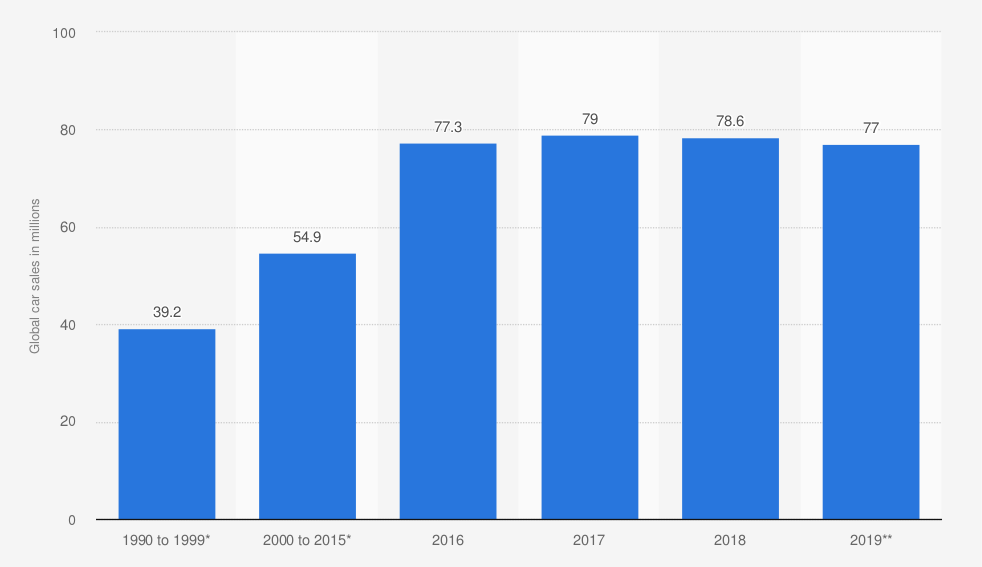
\includegraphics[width=7cm,height=7cm]{img2.png}
    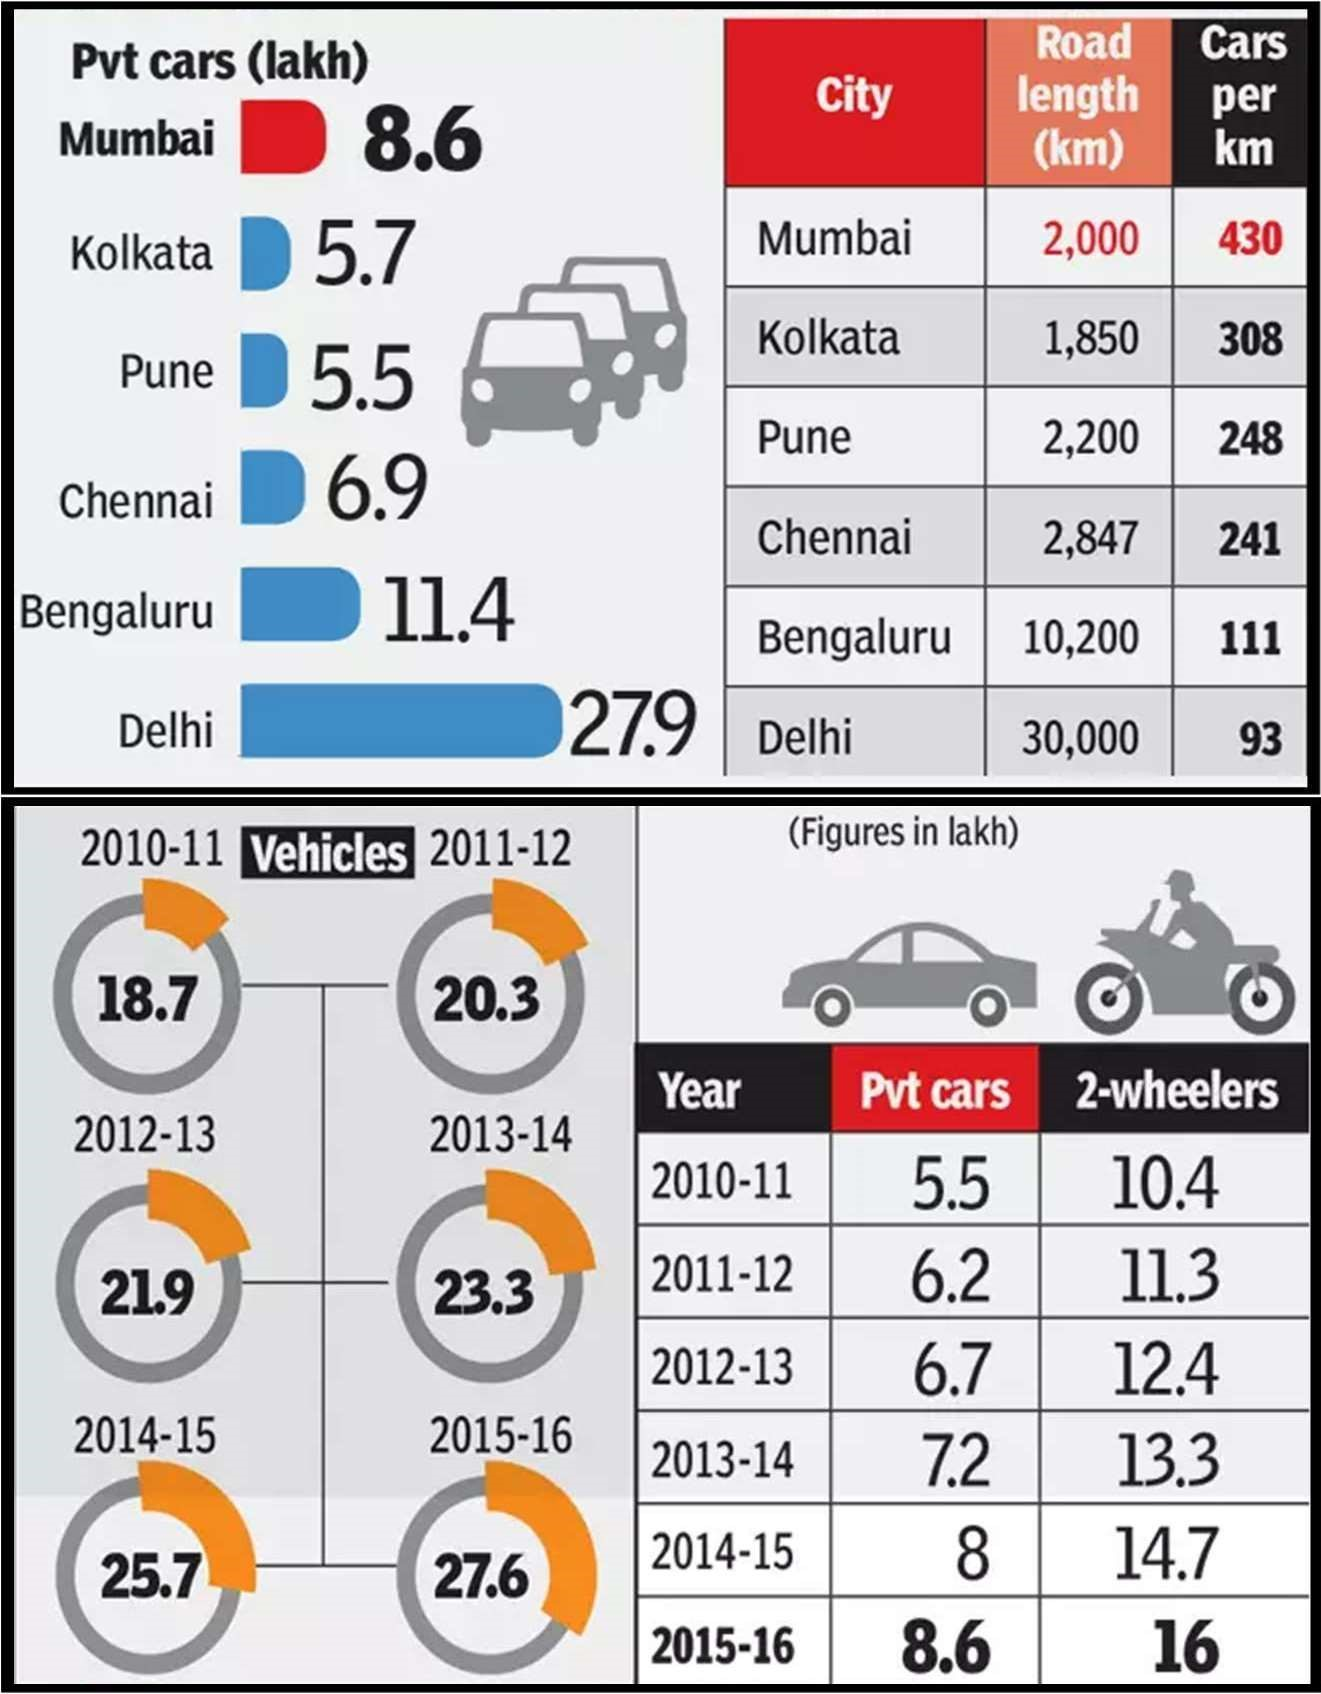
\includegraphics[width=6cm]{img.jpg}
    \end{center}
    \end{figure}

\section[]{Hardware requirements:}
\begin{itemize}
	\item Power Supply (adapters , SMPS etc.)
	\item Arduino
	\item Ultrasonic Sensor/infrared sensor
	\item WiFi module (router)
\end{itemize}

\section{Software requirements:}
\section[]{Hardware requirements:}
\begin{itemize}
	\item Power Supply (adapters , SMPS etc.)
	\item Node MCU
	\item Ultrasonic Sensor
	\item Router
\end{itemize}

\section{Software requirements:}
\begin{itemize}
\item Diptrace
\item Visual Studio code
\item tomcat 7
\item HTML
\item PHP
\item Java Script
\item Cloud
\item CSS - cascade style sheets
\item MySql	
\end{itemize}

\section{Implementation:}
\begin{figure}[ht]
    \centering
    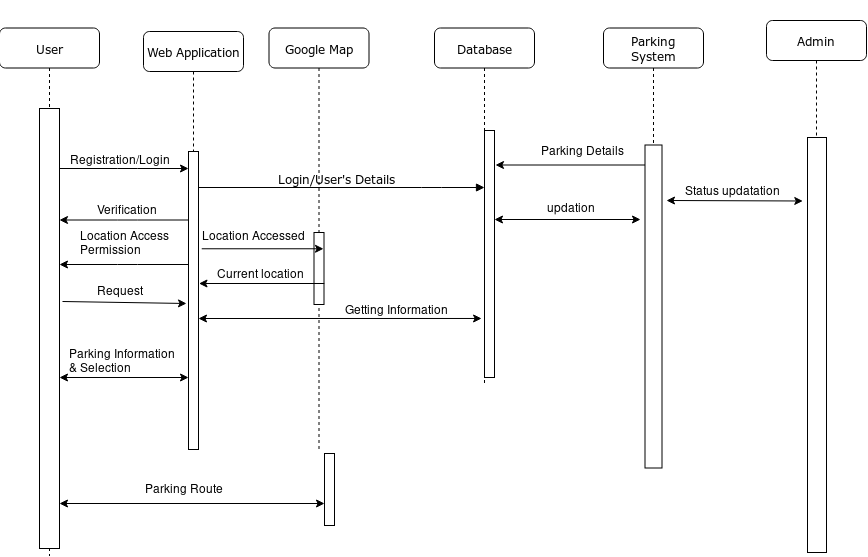
\includegraphics[width=12cm]{i.png}
    \linebreak
    \linebreak
    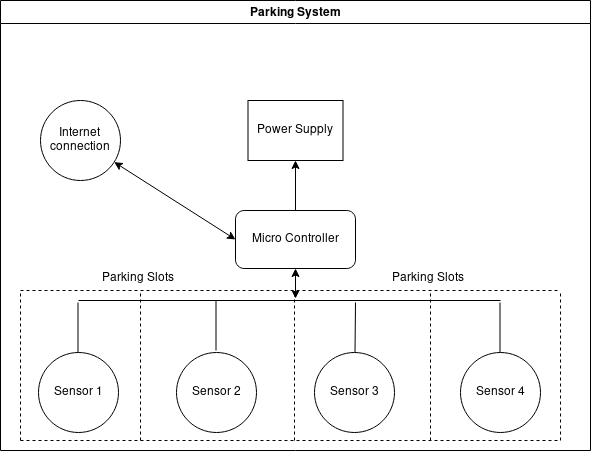
\includegraphics[width=12cm]{i2.png}
    \end{figure}
\subparagraph{The entire project will be made with an effective combination of hardware and software. The major heads in the implementation part are users, a web application, google map, database, a parking system and an admin.}
\subparagraph{\textbf{The User Interface:\newline}
The user is connected and can communicate only with the web application, this could be done for registration or login purpose, verification, location access permission, usage request or for sharing parking information and selection.}
\subparagraph{\textbf{Database:\newline} 
The entire detail of the user is then stored in the database and there is a bidirectional communication between web application and database for transferring information. After getting the permission to access the location, user’s location can be taken with the help of google map and then is stored in the database, thus database now stores every useful information of the user including contact number, email, vehicle registration number, and few more. Database also contains the information and details of the parking systems in the covered zone, and is connected bi-directionally for exchanging updated information.
Admin is also given a bi-directional connectivity with the parking system for providing him/her the status updating.
Finally, the user is connected with the google map and can find directions towards the parking easily.
}
\subparagraph{\textbf{Hardware Structure:\newline}A well-structured parking slots would be made with sensors placed at every slot either in the middle of a slot or according to the available place, each of these sensors are connected to a micro controller. Every lane will have a common micro controller connected with the sensors. These microcontrollers work on power supply therefore the sufficient amount of power supply is also provided to each of them for their proper functionality.}
\subparagraph{
These micro controllers are connected to the internet, basically our database so that they can transmit updated details to the database for proper functioning of this parking management system.
The implementation part with the hardware is cheaper and will provide the best of the ways to solve the parking issues in effective as well in economical ways.
}
\subparagraph{\textbf{\underline{Schedule for implementation: -}}\newline The idea was to create a well organised management system for the available parking spaces in this country, so as to control the traffic hazards occurring due to on road parking. A web application will be made in connectivity with the hardware so that the user can get on-time information about the empty slots and nearby parking space.}
\subparagraph{
The idea was shortlisted for the implementation stage, which encouraged us more to make this idea worth it. We understand the importance of team work and thus the work is equally distributed among ourselves. The team is divided into two halves, one for software part and the other one for hardware part. The distribution is as follows:
}

    \begin{center}
    \begin{tabular}{|l|l|l|}
\hline
 PHASES & DATES & WORK \\
\hline
I & 25 Dec-8 Jan & Structure and final layout of the website \\
\hline
II & 9 Jan-13 Jan & Adding functionality to the website, parallel hardware implementation \\ 
\hline
III & 14 Jan-17 Jan & website-hardware connectivity \\
\hline
IV & 18 Jan-20 Jan & Finishing, final review and testing work \\
\hline
V & 21 Jan- 23 Jan & Video demonstration \\
\hline
VI & 30 Jan & Estimated Submission \\
\hline
    \end{tabular}
    \end{center}
    
\section{Feasibility:}
\subparagraph{Due to the current process of unorganized parking management system, India is facing a problem nowadays – lack of sufficient parking space. With families getting smaller and the total number of motor vehicles exceeding the total number of heads per family, the parking scenario is woefully falling short of the current requirements in the country. The situation is such that on any given working day approximately 40 percent of the roads in urban India are taken up for just parking the cars.}
\subparagraph{In order to overcome these problems and for the ease of peoples, an idea of smart vehicle parking or e-parking system helps users to find a vacant spot using sensors in each parking space by detecting the presence or absence of a vehicle by using a web application. The user can book the slot for parking online which provides ease to the people and it makes our parking management system organized. Due to this organized management, the problems of lack of parking spaces, traffic jams due to parking on road, illegal parking and unorganized management will be solved. Transfer of current unorganized parking system to an organized e-parking system provides an ease to the peoples and provides an advantage of proper traffic management. For the success of this idea, it is required to make awareness among the peoples about this e-parking system and familiar them with use of this system through an online web application.}

\section{References:}
\begin{itemize}
	\item Github
	\item Google
	\item University Suggestion Box
	\item Faculty Guiding
	\item Survey ( Market Research)
\end{itemize}

\end{document}

